\begin{figure*}[!ht]
  \centering
  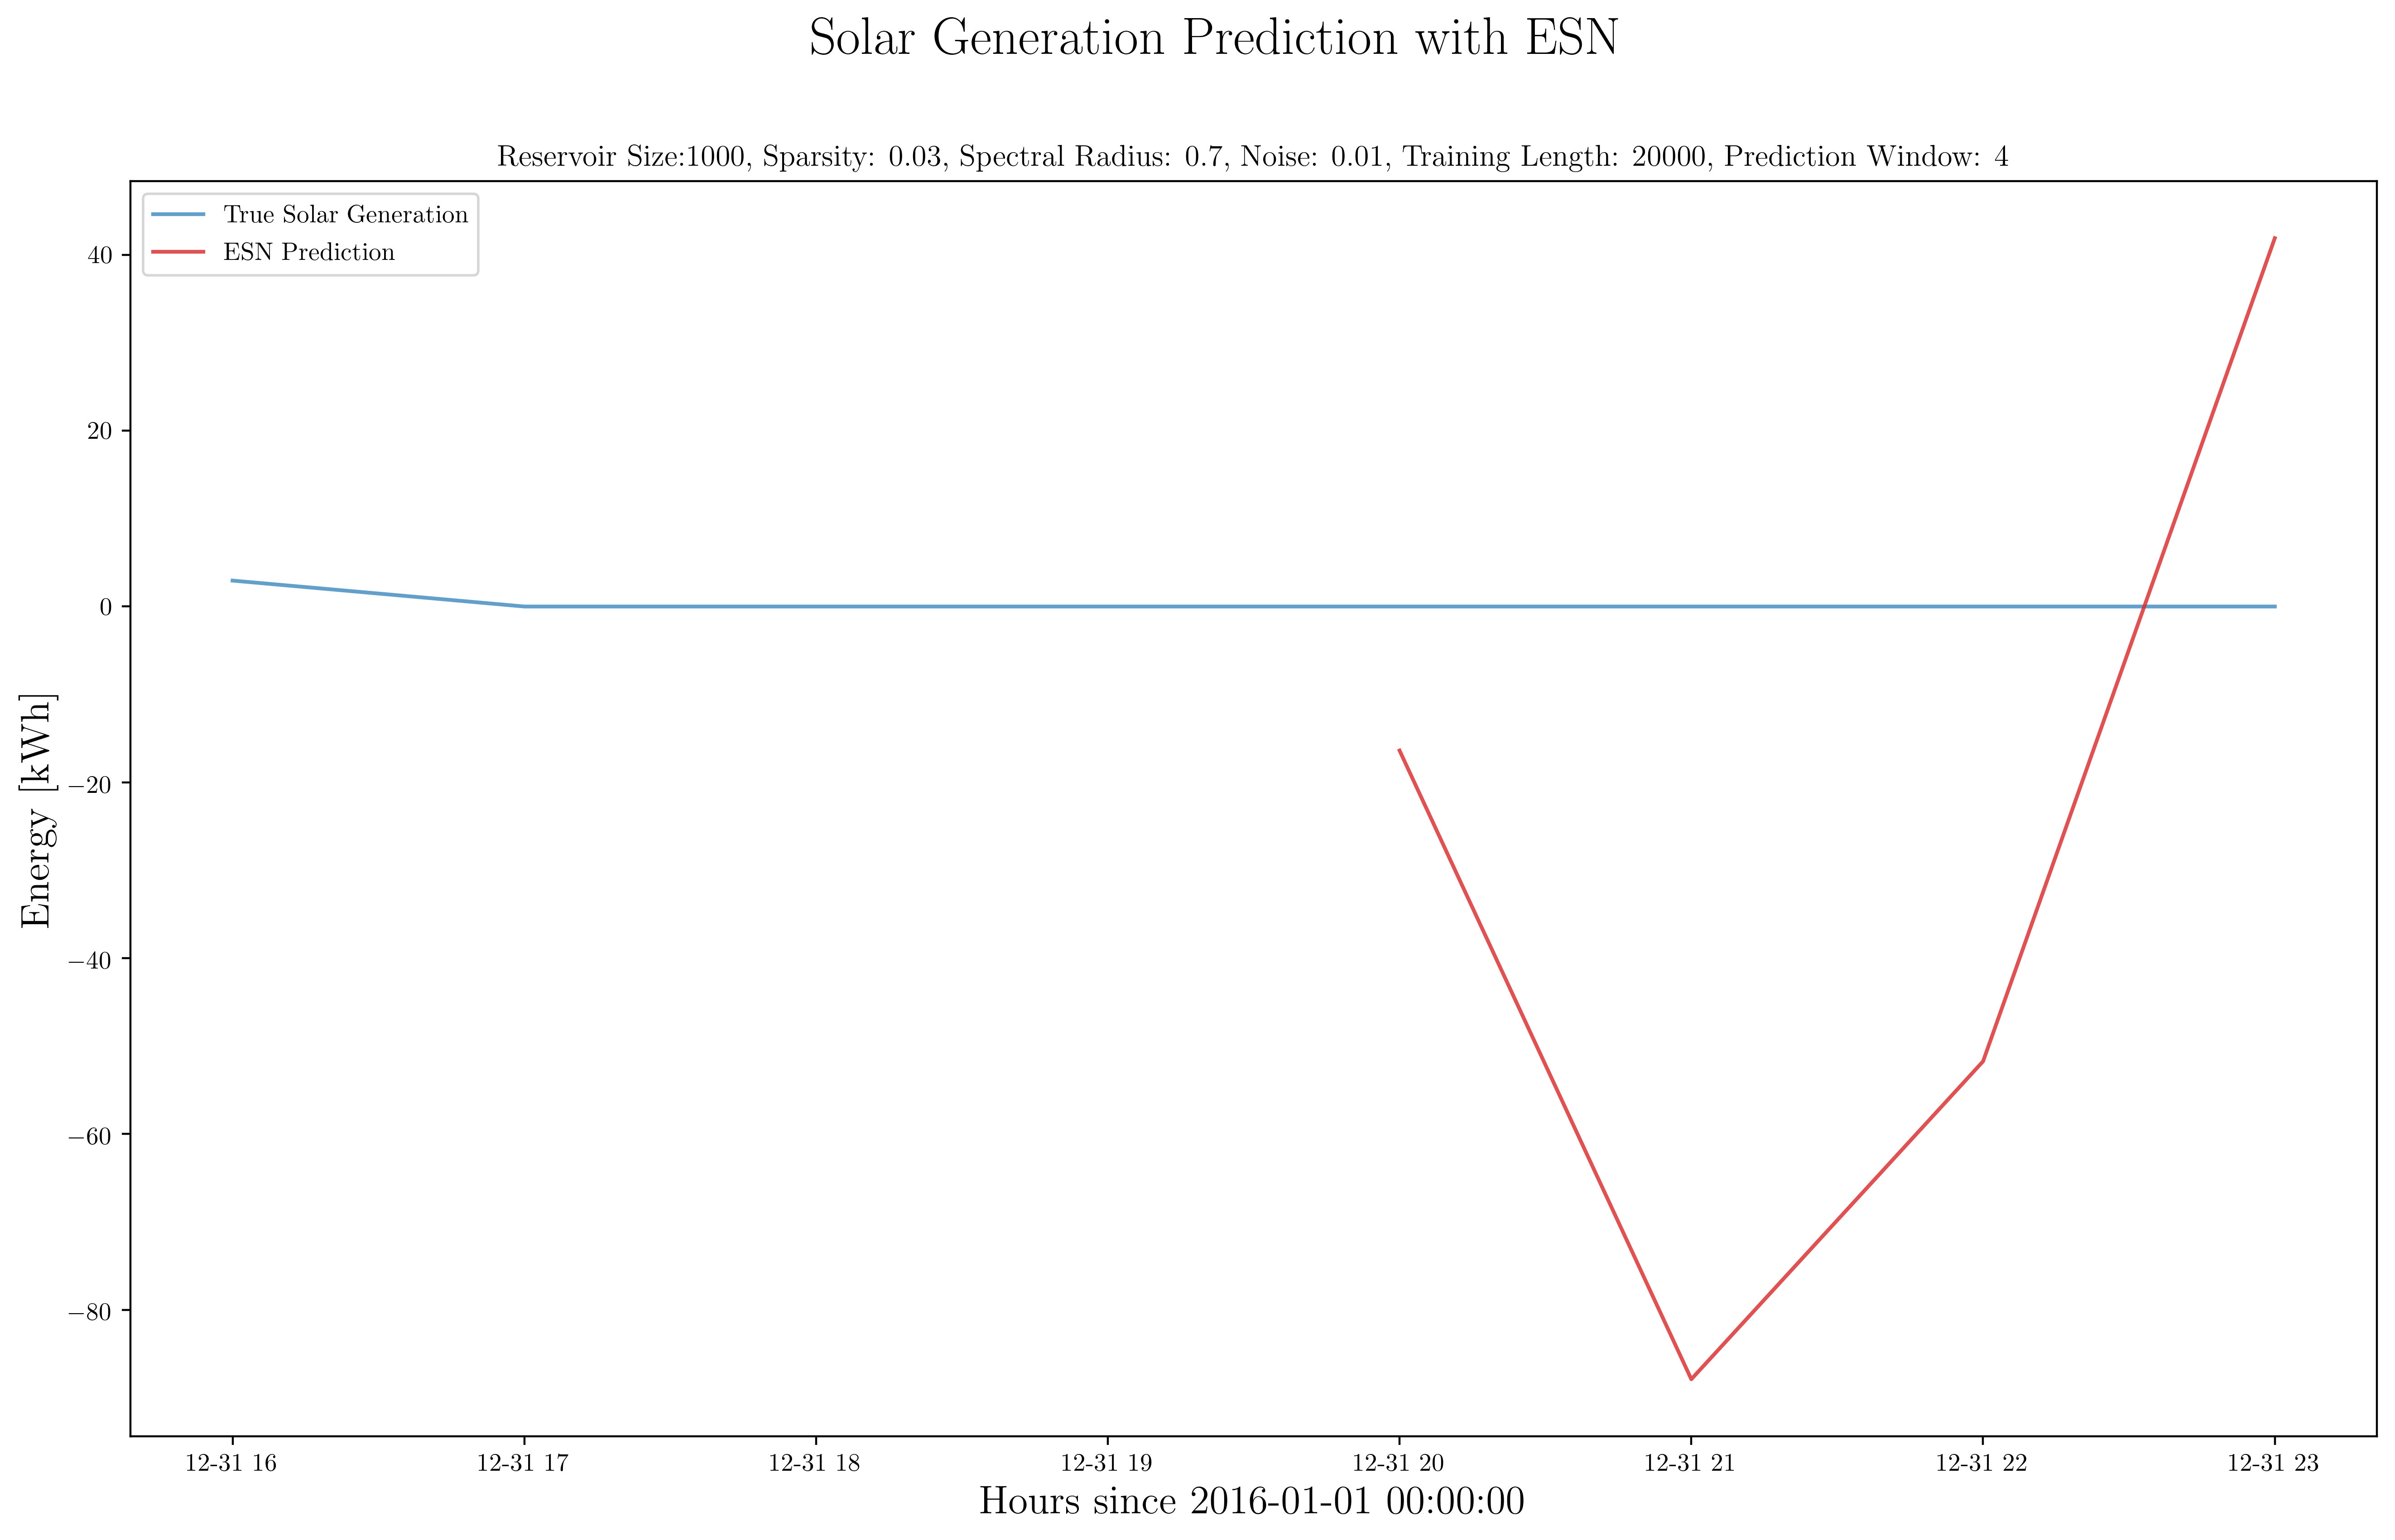
\includegraphics[width=0.8\textwidth]{04_solar_wettemp_prediction.png}
  \caption{The optimized 4 hour ahead solar energy prediction with wet bulb
  temperature as a meteorological predictor.}
  \label{fig:wind04}
\end{figure*}
% \begin{center}
  \begin{table*}[!ht]
    \centering
    \caption{Tabulated error for 4-hour ahead solar energy forecasts with various coupled quantities. Improvement indicates the percentage improvement over the base case of forecasting solar energy alone.}
    \label{tab:solar04}
    \begin{tabular}{l|c|c|c|c}
      &  & & Improvement & Improvement \\
      Scenario  & MAE & RMSE & MAE (\%) & RMSE (\%)\\
      \hline
      Solar Energy & 0.061426 & 0.095794 & [-] & [-] \\
      Solar + Sun Elevation & 0.033263 & 0.060048 & -45.85 & -37.32\\
      Solar + Humidity & 0.054951 & 0.078739 & -10.54& -17.80\\
      Solar + Pressure & 0.046862 & 0.089294 & -23.71& -6.78\\
      Solar + Wet Bulb Temp. & 0.038104 & 0.053419 & -37.97& -44.24\\
      Solar + Dry Bulb Temp. & 0.044104 & 0.073112 & -28.20& -23.68\\
      Solar + Wind Speed & 0.070293 & 0.099912 & +14.44& +4.30\\
    \end{tabular}
  \end{table*}
% \end{center}
